\documentclass[man]{apa6}
\usepackage{lmodern}
\usepackage{amssymb,amsmath}
\usepackage{ifxetex,ifluatex}
\usepackage{fixltx2e} % provides \textsubscript
\ifnum 0\ifxetex 1\fi\ifluatex 1\fi=0 % if pdftex
  \usepackage[T1]{fontenc}
  \usepackage[utf8]{inputenc}
\else % if luatex or xelatex
  \ifxetex
    \usepackage{mathspec}
  \else
    \usepackage{fontspec}
  \fi
  \defaultfontfeatures{Ligatures=TeX,Scale=MatchLowercase}
\fi
% use upquote if available, for straight quotes in verbatim environments
\IfFileExists{upquote.sty}{\usepackage{upquote}}{}
% use microtype if available
\IfFileExists{microtype.sty}{%
\usepackage{microtype}
\UseMicrotypeSet[protrusion]{basicmath} % disable protrusion for tt fonts
}{}
\usepackage{hyperref}
\hypersetup{unicode=true,
            pdftitle={Domain-specific working memory loads selectively increase negative interpretations of surprised facial expressions},
            pdfauthor={Nicholas R. Harp~\& Maital Neta},
            pdfkeywords={ambiguity, working memory, bias},
            pdfborder={0 0 0},
            breaklinks=true}
\urlstyle{same}  % don't use monospace font for urls
\usepackage{graphicx,grffile}
\makeatletter
\def\maxwidth{\ifdim\Gin@nat@width>\linewidth\linewidth\else\Gin@nat@width\fi}
\def\maxheight{\ifdim\Gin@nat@height>\textheight\textheight\else\Gin@nat@height\fi}
\makeatother
% Scale images if necessary, so that they will not overflow the page
% margins by default, and it is still possible to overwrite the defaults
% using explicit options in \includegraphics[width, height, ...]{}
\setkeys{Gin}{width=\maxwidth,height=\maxheight,keepaspectratio}
\IfFileExists{parskip.sty}{%
\usepackage{parskip}
}{% else
\setlength{\parindent}{0pt}
\setlength{\parskip}{6pt plus 2pt minus 1pt}
}
\setlength{\emergencystretch}{3em}  % prevent overfull lines
\providecommand{\tightlist}{%
  \setlength{\itemsep}{0pt}\setlength{\parskip}{0pt}}
\setcounter{secnumdepth}{0}
% Redefines (sub)paragraphs to behave more like sections
\ifx\paragraph\undefined\else
\let\oldparagraph\paragraph
\renewcommand{\paragraph}[1]{\oldparagraph{#1}\mbox{}}
\fi
\ifx\subparagraph\undefined\else
\let\oldsubparagraph\subparagraph
\renewcommand{\subparagraph}[1]{\oldsubparagraph{#1}\mbox{}}
\fi

%%% Use protect on footnotes to avoid problems with footnotes in titles
\let\rmarkdownfootnote\footnote%
\def\footnote{\protect\rmarkdownfootnote}


  \title{Domain-specific working memory loads selectively increase negative interpretations of surprised facial expressions}
    \author{Nicholas R. Harp\textsuperscript{1}~\& Maital Neta\textsuperscript{1}}
    \date{}
  
\shorttitle{DOMAIN-SPECIFIC WORKING MEMORY AND SURPRISED EXPRESSIONS}
\affiliation{
\vspace{0.5cm}
\textsuperscript{1} University of Nebraska-Lincoln}
\keywords{ambiguity, working memory, bias\newline\indent Word count: X}
\usepackage{csquotes}
\usepackage{upgreek}
\captionsetup{font=singlespacing,justification=justified}

\usepackage{longtable}
\usepackage{lscape}
\usepackage{multirow}
\usepackage{tabularx}
\usepackage[flushleft]{threeparttable}
\usepackage{threeparttablex}

\newenvironment{lltable}{\begin{landscape}\begin{center}\begin{ThreePartTable}}{\end{ThreePartTable}\end{center}\end{landscape}}

\makeatletter
\newcommand\LastLTentrywidth{1em}
\newlength\longtablewidth
\setlength{\longtablewidth}{1in}
\newcommand{\getlongtablewidth}{\begingroup \ifcsname LT@\roman{LT@tables}\endcsname \global\longtablewidth=0pt \renewcommand{\LT@entry}[2]{\global\advance\longtablewidth by ##2\relax\gdef\LastLTentrywidth{##2}}\@nameuse{LT@\roman{LT@tables}} \fi \endgroup}


\DeclareDelayedFloatFlavor{ThreePartTable}{table}
\DeclareDelayedFloatFlavor{lltable}{table}
\DeclareDelayedFloatFlavor*{longtable}{table}
\makeatletter
\renewcommand{\efloat@iwrite}[1]{\immediate\expandafter\protected@write\csname efloat@post#1\endcsname{}}
\makeatother
\usepackage{lineno}

\linenumbers

\authornote{Nicholas R. Harp, Department of Psychology, Center for Brain, Biology, and Behavior, University of Nebraska-Lincoln
Maital Neta, Department of Psychology, Center for Brain, Biology, and Behavior, University of Nebraska-Lincoln

Correspondence concerning this article should be addressed to Nicholas R. Harp, Postal address. E-mail: \href{mailto:nharp@huskers.unl.edu}{\nolinkurl{nharp@huskers.unl.edu}}}

\abstract{
Individual differences in interpretations of emotional ambiguity are a useful tool for measuring affective biases.

While trait-like, these biases are also susceptible to experimental manipulations. In the present study, we capitalize on this malleability to expand on previous research suggesting that
subjective interpretations are stable independently of cognitive load.

We tested the effects of working memory loads containing either neutral or emotional content on concurrent interpretations of surprised facial expressions.

Here we show that interpretations of surprise are more negative during maintenance of working memory loads with emotional content compared to those with neutral content.

Two or three sentences explaining what the \textbf{main result} reveals in direct comparison to what was thought to be the case previously, or how the main result adds to previous knowledge.

One or two sentences to put the results into a more \textbf{general context}.

Two or three sentences to provide a \textbf{broader perspective}, readily comprehensible to a scientist in any discipline.


}

\begin{document}
\maketitle

\hypertarget{introduction}{%
\section{Introduction}\label{introduction}}

\hypertarget{facial-expressions-and-individual-differences}{%
\subsection{Facial expressions and individual differences}\label{facial-expressions-and-individual-differences}}

Facial expressions are important social signals, often communicating emotion between individuals and even sparking emotional responses in the perceiver (Frith, 2009). Researchers have long argued that facial expressions are universal signals of emotion, positing humans' innate ability to associate facial expressions with emotional experience (Darwin, 1872; Ekman \& Friesen, 1971; Izard, 1994). More recently, Barrett and colleagues suggested that the relationship between facial expressions and emotions is more complex, stating that expression of an emotion may vary across cultures, social context, or even individuals (Barrett, Adolphs, Marsella, Martinez, \& Pollak, 2019). Other work has shown individual differences in interpretations of facial expressions (Green \& Guo, 2018; Neta, Norris, \& Whalen, 2009). Regardless of this variability in emotional expressions, experience, and interpretations, humans readily make judgments about personality traits (e.g., trustworthiness), aesthetics (e.g., attractiveness), and emotions from faces (Carroll \& Russell, 1996; Said \& Todorov, 2011; Todorov, Baron, \& Oosterhof, 2008). Interpretations of valence (i.e., the inherent positive or negative emotional value of a stimulus) are one instance of judgments of facial expressions guiding potential social (i.e., approach-avoidance) behavior (Krieglmeyer, Deutsch, De Houwer, \& De Raedt, 2010).

While most people can accurately differentiate the emotional valence of many facial expressions, such as consistently interpreting angry (happy) faces as negative (positive), there are individual differences in valence judgments of emotionally ambiguous facial expressions, like a surprised face (Neta et al., 2009; Petro, Tong, Henley, \& Neta, 2018 ). This difference in valence interpretations of surprised expressions is attributable to such stimuli's predictive value for both positive and negative outcomes in an individual's previous experience. For instance, a surprised expression could signal positive (e.g., winning the lottery) or negative (e.g., a car accident) events. These differences in valence interpretations represent an important individual difference, as the same stimulus can result in two alternative interpretations between individuals--likely leading to different downstream behaviors (e.g., Krieglmeyer et al., 2010). This individual difference in interpretations of emotionally ambiguous stimuli is known as one's \emph{valence bias}, and a growing body of work has used both facial expressions and scenes to better understand this individual difference (Neta, Kelley, \& Whalen, 2013; Neta et al., 2009; Neta \& Whalen, 2010).

Despite one's valence bias, the initial response to ambiguity appears to be negativity (Neta, Davis, \& Whalen, 2011; Neta et al., 2009; Neta \& Whalen, 2010; Petro et al., 2018). Under this framework, which is known as the \emph{initial negativity} hypothesis, positive interpretations rely on the implementation of some emotion regulation strategy, perhaps similar to cognitive reappraisal. During cognitive reappraisal, individuals work to change intial perceptions of an emotional stimulus (Lazarus \& Alfert, 1964). Similarly, the initial negativity hypothesis posits that individuals' initial perception of surprised expressions is negative, and that those arriving at a positive interpretation must implement a regulatory mechanism to alter their interpretation.

Behavioral evidence supports the initial negativity hypothesis. For instance, reaction time data show that individuals with more positive biases take longer to reach a valence judgment for surprised expressions than those with a more negative bias (Neta et al., 2009), suggesting a more time-intensive (regulatory) process for positive interpretations. Other work demonstrates the faster and default nature of negative interpretations through presenting either low- (LSF) or high-spatial frequency (HSF) images of surprised expressions. The images with only LSF information, which is processed earlier than its HSF counterpart, were rated more negatively than the HSF images (Neta \& Whalen, 2010). Additionally, surprised facial expressions are more quickly detected in an emotional oddball paradigm among happy (positive) than angry (negative) faces (Neta et al., 2011). The results from this paradigm suggest that surprised expressions are more readily perceived as similar to angry faces (i.e., perceived as negative) than happy faces.

There is also support for the initial negativity hypothesis in neuroimaging studies. Ventromedial prefrontal cortex, a putative regulatory region, and amygdala actively are inversely correlated, and participants with more negative biases show higher activity in the amygdala while more positive participants show higher activity in vmPFC (Kim, Somerville, Johnstone, Alexander, \& Whalen, 2003). More recently, Petro and colleagues (2018) showed that participants with a more positive valence bias show more activity for surprised faces in emotion regulation-related brain regions (vmPFC).Taken together, both behavioral and brain data support the notion that negative interpretations of surprised faces are a faster, default process and positive interpretations rely on slower regulatory processes, which may be susceptible to demands from other cognitive processes.

\hypertarget{cognitive-loads-and-task-interference}{%
\subsection{Cognitive loads and task interference}\label{cognitive-loads-and-task-interference}}

In daily life, cognitive resources are often shared among several processes as stimuli compete for our attention. For example, imagine a student attending a lecture. If the student is frequently distracted by notifications and directing cognitive resources towards a text message conversation, computer applications, or even daydreams, then the student's ability to understand and remember the lecture will likely suffer. Indeed, cognitive resource competition, a phenomenon known as cognitive load, negatively impacts executive processes, such as attention (Lavie, Hirst, Fockert, \& Viding, 2004; Murphy, Groeger, \& Greene, 2016). High levels of cognitive load alter performance on a variety of tasks, including those in both cognitive and emotional domains (Kron, Schul, Cohen, \& Hassin, 2010; Nagamatsu et al., 2011; Pontari \& Schlenker, 2000, @jiaping\_empathy\_2017; Thomas, Donohue-Porter, \& Stein Fishbein, 2017). Working memory tasks, which require participants to maintain some stimulus representation in working memory, are often used for testing cognitive load effects (e.g., Burnham, 2010, @lavie\_role\_2005, or see @murphy\_twenty\_2016 for a review).

The cognitive demands of active working memory maintenance often interact with concurrent affective processes (e.g., face categorization, subjective emotional experience), perhaps as a result of a shared resource pool for these processes. For instance, Ahmed (2018) showed that performance on a facial expression categorization task suffers when participants are under high cognitive load. Other work has linked cognitive load to changes in emotional responses (Blair et al., 2007; Van Dillen, Heslenfeld, \& Koole, 2009). For example, higher loads during a working memory task reduce subjective emotional experience, as well as amygdala activity (Van Dillen et al., 2009). Other neuroimaging work has shown that Stroop interference effects were exaggerated during trials temporally surrounded by emotional stimuli, while emotional responses in the brain (i.e., amygdala and inferior frontal gyrus activation) were lower during trials with Stroop task demands compared to trials with no concurrent task demands (Blair et al., 2007). Other work highlights the importance of cognitive load task characteristics on a syllogistic reasoning task, demonstrating that participants perform worse on tasks with emotional, rather than neutral, content when under high cognitive load (Trémolière, Gagnon, \& Blanchette, 2016). Together, these effects suggest an overlap between cognitive demands and emotional processes, with high cognitive demands interfering with typical emotion processing.

Previous work has tested the effects of cognitive load on valence bias to assess both subjective ratings of surprise and the underlying cognitive-motor dynamics of the ratings via mousetracking. While there was no effect of load on subjective interpretations of surprised expressions, participants did show altered mouse trajectories, such that mouse movements were less drawn towards the response option (i.e., positive or negative) in line with one's bias (Mattek, Whalen, Berkowitz, \& Freeman, 2016). One potential explanation for the null effect of load on ratings is the domain-specificity of the cognitive load. While there are some domain-general effects of cognitive load on emotional processing (Blair et al., 2007; Van Dillen et al., 2009), which helps explain the effects of load on mouse trajectories, other lines of work have shown dissociable processing of emotional and non-emotional task stimuli (Egner, Etkin, Gale, \& Hirsch, 2008). Critically, Mattek and colleagues (2016) used non-emotional stimuli (i.e., number sequence) in their manipulation of cognitive load during interpretations of surprised facial expressions. The cognitive demand required for maintaining emotional information in working memory may tax resources used for emotion regulation more so than non-emotional information. Under the initial negativity framework, this would lead to more negative interpretations of surprise during cognitive load with emotional stimuli.

\hypertarget{the-present-study}{%
\subsection{The present study}\label{the-present-study}}

In the present study we test the effects of both low and high cognitive load across emotional and non-emotional domains. We expect to find a main effect of load domain, emotional or non-emotional, on interpretations of surprise, such that interpretations made under emotional working memory loads are more negative than those made under non-emotional working memory loads. Further, we predict an interaction effect, such that emotional working memory loads with more content (high load) will result in more negative interpetations than emotional working memory loads with less content (low load).

\hypertarget{methods}{%
\section{Methods}\label{methods}}

\hypertarget{participants}{%
\subsection{Participants}\label{participants}}

Fifty-eight subjects were recruited from the undergraduate research pool at the University of Nebraska-Lincoln. The data from eight subjects were excluded due to technical difficulties resulting from an error in one of the experiment scripts. This left 50 individuals in the final sample for analysis. The mean age of the remaining sample was 18.82 (1.19), a majority of participants were female (82.00\%), and all were white/caucasian without hispanic/Latinx ethnicity. All subjects provided written informed consent in accordance with the Declaration of Helsinki and all procedures were approved by the University of Nebraska-Lincoln Institutional Review Board (Approval \#20141014670EP). Each participant received course credit for completing the study.

\hypertarget{material}{%
\subsection{Material}\label{material}}

\hypertarget{stimuli}{%
\subsubsection{Stimuli}\label{stimuli}}

The stimuli included faces from the NimStim (Tottenham et al., 2009) and Karolinska Directed Emotional Faces (Lundqvist, Flykt, \& Öhman, 1998) stimuli sets, as in previous work (Brown, Raio, \& Neta, 2017; Neta \& Whalen, 2010). The faces consisted of 34 unique identities including 11 angry, 12 happy, and 24 surprised expressions organized pseudorandomly. The scene stimuli were selected from the International Affective Picture System (Lang, Bradley, \& Cuthbert, 2008). A total of 288 scenes (72 positive, 72 negative, and 144 neutral) were selected for the image matrices. The positive and negative images did not differ on arousal (Z = -0.23, p = 0.82). The scenes were organized into low (two images) and high (six images) cognitive load of either neutral or emotional (equal number of positive and negative) images (Figure 1).

\hypertarget{procedure}{%
\subsection{Procedure}\label{procedure}}

After arriving at the lab, participants provided informed consent prior to completing the task. Participants were randomly assigned to complete one of the task versions, which included 144\footnote{Some versions of the task only included 142 trials due to a programming error.} trials split between working memory probe and face rating trials. The task was completed using MouseTracker software (Freeman \& Ambady, 2010) and participants responded with a mouse to indicate the appropriate response for the face ratings (i.e., \enquote{POSITIVE} or \enquote{NEGATIVE}) and the memory probe (i.e., \enquote{YES} or \enquote{NO}). The trials were self-initiated; that is, the participant clicked a \enquote{start} button at the bottom of the screen at the beginning of each trial at their own pace. After initiating the trial, a fixation cross appeared (1000 ms), then participants viewed an image matrix, which the participants were instructed to remember for the duration of the trial. The image matrix was presented for 4000 ms and the image was either a low or high load matrix consisting of either emotional (equal positive and negative) or neutral images. After the image matrix a happy, angry, or surprised face appeared for 1000 ms and the participants rated the face by clicking on either the positive or negative response option. After the face rating, a single image probe appeared (5000 ms), and participants indicated whether or not the image probe was present in the previous image matrix.

\hypertarget{data-analysis}{%
\subsection{Data analysis}\label{data-analysis}}

We used R (Version 3.6.0; {\textbf{???}}) and the R-packages * \}dplyr* {[}@ \}R-dplyr{]}, \emph{BayesFactor} (Version 0.9.12.4.2; {\textbf{???}}), \emph{broom} (Version 0.5.2; {\textbf{???}}), \emph{circlize} (Version 0.4.6; {\textbf{???}}), \emph{coda} (Version 0.19.2; {\textbf{???}}), \emph{cstab} (Version 0.2.2; {\textbf{???}}), \emph{diptest} (Version 0.75.7; {\textbf{???}}), \emph{dotCall64} (Version 1.0.0; {\textbf{???}}; {\textbf{???}}), \emph{fastcluster} (Version 1.1.25; {\textbf{???}}), \emph{fields} (Version 9.8.3; {\textbf{???}}), \emph{forcats} (Version 0.4.0; {\textbf{???}}), \emph{foreach} (Version 1.4.7; {\textbf{???}}), \emph{ggplot2} (Version 3.1.1; {\textbf{???}}), \emph{jpeg} (Version 0.1.8; {\textbf{???}}), \emph{lattice} (Version 0.20.38; {\textbf{???}}), \emph{magrittr} (Version 1.5; {\textbf{???}}), \emph{maps} (Version 3.3.0; {\textbf{???}}), \emph{Matrix} (Version 1.2.17; {\textbf{???}}), \emph{mousetrap} (Version 3.1.2; {\textbf{???}}), \emph{openxlsx} (Version 4.1.0; {\textbf{???}}), \emph{papaja} (Version 0.1.0.9842; {\textbf{???}}), \emph{plyr} (Version 1.8.4; @ \}R-dplyr; {\textbf{???}}), \emph{pracma} (Version 2.2.5; {\textbf{???}}), \emph{processx} (Version 3.3.1; {\textbf{???}}), \emph{psych} (Version 1.8.12; {\textbf{???}}), \emph{purrr} (Version 0.3.2; {\textbf{???}}), \emph{RColorBrewer} (Version 1.1.2; {\textbf{???}}), \emph{Rcpp} (Version 1.0.1; {\textbf{???}}; {\textbf{???}}), \emph{readbulk} (Version 1.1.2; {\textbf{???}}), \emph{readr} (Version 1.3.1; {\textbf{???}}), \emph{readxl} (Version 1.3.1; {\textbf{???}}), \emph{Rmisc} (Version 1.5; {\textbf{???}}), \emph{scales} (Version 1.0.0; {\textbf{???}}), \emph{spam} (Version 2.2.2; {\textbf{???}}; {\textbf{???}}; {\textbf{???}}), \emph{stringr} (Version 1.4.0; {\textbf{???}}), \emph{tibble} (Version 2.1.3; {\textbf{???}}), \emph{tidyr} (Version 0.8.3.9000; {\textbf{???}}), \emph{tidyverse} (Version 1.2.1; {\textbf{???}}), and \emph{yarrr} (Version 0.1.5; {\textbf{???}}) for all our analyses. Data preprocessing was completed in R using the mousetrap package ({\textbf{???}}). First, percent negative ratings were calculated for happy, angry, and surprised faces across all trial types, as well as a percent correct score for the memory probe trials. After, trials were screened for RT outliers. Any trials that were greater than three standard deviations from the mean were removed from the analyses. Additionally, we removed the preceding face rating trial for any incorrect memory probe trials, as these trials can be considered a manipulation failure.

Prior to completing the analyses, all data were assessed for normality using Shapiro-Wilks tests. We tested for differences in valence bias among the different working memory load conditions. Friedman's test was used to assess overall differences and pairwise comparisons were completed using Wilcoxon signed rank tests using Bonferroni correction. Next, we tested for differences among maximum deviations in each working memory load condition using a load (low, high) X domain (emotional, neutral) repeated-measures ANOVA.

\hypertarget{results}{%
\section{Results}\label{results}}

\hypertarget{subjective-ratings}{%
\subsection{Subjective ratings}\label{subjective-ratings}}

Distributions of ratings were first tested for normality using Shapiro-Wilk's test. The results of all four tests were highly significant (p's \textless{} .001), so non-parametric tests were used for data analysis. Friedman's test results showed significantly different rank-order distributions across the conditions \(\chi^{2}\)(3.00) = 27.79, p \textless{} .001. Follow up Wilcoxon signed rank tests revealed that surprise is rated as more negative when holding emotional content in working memory compared to neutral content, and this was true for both low and high loads. Low emotional load ratings were significantly more negative than low, Z = 3.27, p = .001, neutral and high, Z = 3.67, p \textless{} .001, neutral loads. The same was true for high emotional load ratings and low, Z = 4.55, p \textless{} .001, and high, Z = 3.81, p \textless{} .001, neutral loads. However, there was no effect of load. That is, the comparisons between low and high load ratings for both emotional, Z = -1.35, p = .176, and neutral, Z = -0.06, p = .954, load ratings were not significantly different.\footnote{These results are qualitatively the same when analyzing these data with a repeated measures ANOVA.}
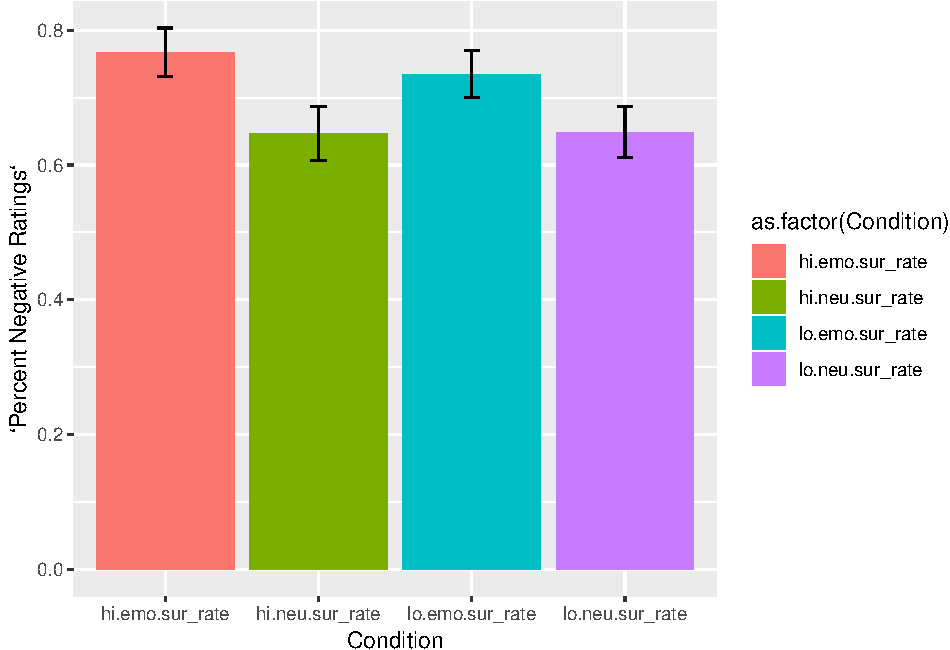
\includegraphics{Manuscript_files/figure-latex/plot figure 1-1.pdf}

Next, we assessed differences in maximum absolute deviation (MD) across the working memory trial conditions. While one of the conditions, low emotional MD, was not normally distributed (p = .024), all other conditions were normally distributed and repeated-measures ANOVA was used to analyze the MDs across conditions. There was a significant effect of load, F(1.00,196.00) = 5.51, p = .020, such that MDs under high load were larger than trials with low load. There was no significant effect of domain on MDs, F(1.00 196.00) = 0.01, p = .912, nor an interaction of load by domain, F(1.00 196.00) = 0.00, p = .960.
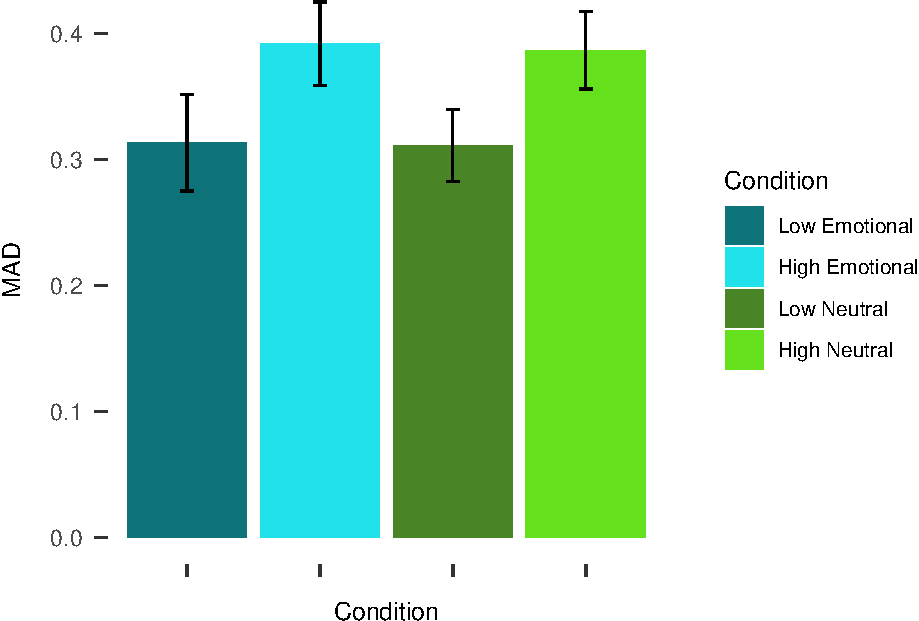
\includegraphics{Manuscript_files/figure-latex/MAD plot-1.pdf}

\hypertarget{discussion}{%
\section{Discussion}\label{discussion}}

The effect of high vs.~low load is still not apparent in these data, just like Mattek et al.~2016. An alternative explanation is that the high load manipulation is not sufficiently difficult to recruit the targeted cognitive resources; however, future work will be needed to better test this alternative.

Increased working memory demands (i.e., a higher cognitive load) do not always result in poorer performance on concurrent tasks. For instance Baddeley -(Baddeley, 1986) reported that increasing load by adding digits to a rehearsed number did not affect accuracy on a concurrent verbal reasoning task--instead, there was an increase in the latency of response, a potential interference effect that did not alter overall accuracy.

Previous work has shown that more positive interpretations of surprised faces are related to slower RTs. Our working hypothesis suggests that this delayed reaction is a result of deliberation and slower, top-down cognitive processing. It is interesting to note that, at least in these data, there is no such difference observed between the neutral and emotional WM trials, \emph{even though} the emotional WM trials are overall more negative. Future work should tease apart why this may be. For instance, \ldots{}

Future work should consider whether the representations of these emotional images in AWM (Reuter-Lorenz), or

\newpage

\hypertarget{references}{%
\section{References}\label{references}}

\begingroup
\setlength{\parindent}{-0.5in}
\setlength{\leftskip}{0.5in}

\hypertarget{refs}{}
\leavevmode\hypertarget{ref-ahmed_knowing_2018}{}%
Ahmed, L. (2018). Knowing how you are feeling depends on what's on my mind: Cognitive load and expression categorization. \emph{Emotion}, \emph{18}(2), 190--201. doi:\href{https://doi.org/10.1037/emo0000312}{10.1037/emo0000312}

\leavevmode\hypertarget{ref-baddeley_working_1986}{}%
Baddeley, A. D. (1986). Working memory. \emph{Philosophical Transactions of the Royal Society of London}, \emph{302}(110), 311--324.

\leavevmode\hypertarget{ref-barrett_emotional_2019}{}%
Barrett, L. F., Adolphs, R., Marsella, S., Martinez, A. M., \& Pollak, S. D. (2019). Emotional expressions reconsidered: Challenges to inferring emotion from human facial movements. \emph{Psychological Science in the Public Interest: A Journal of the American Psychological Society}, \emph{20}(1), 1--68. doi:\href{https://doi.org/10.1177/1529100619832930}{10.1177/1529100619832930}

\leavevmode\hypertarget{ref-blair_modulation_2007}{}%
Blair, K. S., Smith, B. W., Mitchell, D. G. V., Morton, J., Vythilingam, M., Pessoa, L., \ldots{} Blair, R. J. R. (2007). Modulation of emotion by cognition and cognition by emotion. \emph{NeuroImage}, \emph{35}(1), 430--440. doi:\href{https://doi.org/10.1016/j.neuroimage.2006.11.048}{10.1016/j.neuroimage.2006.11.048}

\leavevmode\hypertarget{ref-brown_cortisol_2017}{}%
Brown, C. C., Raio, C. M., \& Neta, M. (2017). Cortisol responses enhance negative valence perception for ambiguous facial expressions. \emph{Scientific Reports}, \emph{7}(1), 15107. doi:\href{https://doi.org/10.1038/s41598-017-14846-3}{10.1038/s41598-017-14846-3}

\leavevmode\hypertarget{ref-burnham_cognitive_2010}{}%
Burnham, B. R. (2010). Cognitive load modulates attentional capture by color singletons during effortful visual search. \emph{Acta Psychologica}, \emph{135}(1), 50--58. doi:\href{https://doi.org/10.1016/j.actpsy.2010.05.003}{10.1016/j.actpsy.2010.05.003}

\leavevmode\hypertarget{ref-carroll_facial_1996}{}%
Carroll, J. M., \& Russell, J. A. (1996). Do facial expressions signal specific emotions? Judging emotion from the face in context. \emph{Journal of Personality and Social Psychology}, \emph{70}(2), 205--218. doi:\href{https://doi.org/10.1037//0022-3514.70.2.205}{10.1037//0022-3514.70.2.205}

\leavevmode\hypertarget{ref-darwin_expression_1872}{}%
Darwin, C. (1872). \emph{The expression of the emotions in man and animals}. John Murray.

\leavevmode\hypertarget{ref-egner_dissociable_2008}{}%
Egner, T., Etkin, A., Gale, S., \& Hirsch, J. (2008). Dissociable neural systems resolve conflict from emotional versus nonemotional distracters. \emph{Cerebral Cortex (New York, N.Y.: 1991)}, \emph{18}(6), 1475--1484. doi:\href{https://doi.org/10.1093/cercor/bhm179}{10.1093/cercor/bhm179}

\leavevmode\hypertarget{ref-ekman_constants_1971}{}%
Ekman, P., \& Friesen, W. V. (1971). Constants across cultures in the face and emotion. \emph{Journal of Personality and Social Psychology}, \emph{17}(2), 124--129. doi:\href{https://doi.org/10.1037/h0030377}{10.1037/h0030377}

\leavevmode\hypertarget{ref-freeman_mousetracker:_2010}{}%
Freeman, J. B., \& Ambady, N. (2010). MouseTracker: Software for studying real-time mental processing using a computer mouse-tracking method. \emph{Behavior Research Methods}, \emph{42}(1), 226--241. doi:\href{https://doi.org/10.3758/BRM.42.1.226}{10.3758/BRM.42.1.226}

\leavevmode\hypertarget{ref-frith_role_2009}{}%
Frith, C. (2009). Role of facial expressions in social interactions. \emph{Philosophical Transactions of the Royal Society B: Biological Sciences}, \emph{364}(1535), 3453--3458. doi:\href{https://doi.org/10.1098/rstb.2009.0142}{10.1098/rstb.2009.0142}

\leavevmode\hypertarget{ref-green_factors_2018}{}%
Green, C., \& Guo, K. (2018). Factors contributing to individual differences in facial expression categorisation. \emph{Cognition \& Emotion}, \emph{32}(1), 37--48. doi:\href{https://doi.org/10.1080/02699931.2016.1273200}{10.1080/02699931.2016.1273200}

\leavevmode\hypertarget{ref-izard_innate_1994}{}%
Izard, C. E. (1994). Innate and universal facial expressions: Evidence from developmental and cross-cultural research. \emph{Psychological Bulletin}, \emph{115}(2), 288--299. doi:\href{https://doi.org/10.1037/0033-2909.115.2.288}{10.1037/0033-2909.115.2.288}

\leavevmode\hypertarget{ref-jiaping_empathy_2017}{}%
Jiaping, C., Yuejia, L. U. O., Fang, C. U. I., Jiaping, C., Yuejia, L. U. O., \& Fang, C. U. I. (2017). Empathy for pain influenced by cognitive load: Evidence from an ERP study. \emph{Acta Psychologica Sinica}, \emph{49}(5), 622--630. doi:\href{https://doi.org/10.3724/SP.J.1041.2017.00622}{10.3724/SP.J.1041.2017.00622}

\leavevmode\hypertarget{ref-kim_inverse_2003}{}%
Kim, H., Somerville, L. H., Johnstone, T., Alexander, A. L., \& Whalen, P. J. (2003). Inverse amygdala and medial prefrontal cortex responses to surprised faces. \emph{Neuroreport}, \emph{14}(18), 2317--2322. doi:\href{https://doi.org/10.1097/00001756-200312190-00006}{10.1097/00001756-200312190-00006}

\leavevmode\hypertarget{ref-krieglmeyer_being_2010}{}%
Krieglmeyer, R., Deutsch, R., De Houwer, J., \& De Raedt, R. (2010). Being moved: Valence activates approach-avoidance behavior independently of evaluation and approach-avoidance intentions. \emph{Psychological Science}, \emph{21}(4), 607--613. doi:\href{https://doi.org/10.1177/0956797610365131}{10.1177/0956797610365131}

\leavevmode\hypertarget{ref-kron_feelings_2010}{}%
Kron, A., Schul, Y., Cohen, A., \& Hassin, R. R. (2010). Feelings don't come easy: Studies on the effortful nature of feelings. \emph{Journal of Experimental Psychology: General}, \emph{139}(3), 520--534. doi:\href{https://doi.org/10.1037/a0020008}{10.1037/a0020008}

\leavevmode\hypertarget{ref-lang_international_2008}{}%
Lang, P., Bradley, M. M., \& Cuthbert, B. N. (2008). International affective picture system (IAPS): Affective ratings of pictures and instruction manual., Technical Report A--8. University of Florida, Gainesville, FL.

\leavevmode\hypertarget{ref-lavie_role_2005}{}%
Lavie, N., \& De Fockert, J. (2005). The role of working memory in attentional capture. \emph{Psychonomic Bulletin \& Review}, \emph{12}(4), 669--674. doi:\href{https://doi.org/10.3758/BF03196756}{10.3758/BF03196756}

\leavevmode\hypertarget{ref-lavie_load_2004}{}%
Lavie, N., Hirst, A., Fockert, J. W. de, \& Viding, E. (2004). Load theory of selective attention and cognitive control. \emph{Journal of Experimental Psychology. General}, \emph{133}(3), 339--354. doi:\href{https://doi.org/10.1037/0096-3445.133.3.339}{10.1037/0096-3445.133.3.339}

\leavevmode\hypertarget{ref-lazarus_short-circuiting_1964}{}%
Lazarus, R. S., \& Alfert, E. (1964). Short-circuiting of threat by experimentally altering cognitive appraisal. \emph{The Journal of Abnormal and Social Psychology}, \emph{69}(2), 195--205. doi:\href{https://doi.org/10.1037/h0044635}{10.1037/h0044635}

\leavevmode\hypertarget{ref-lundqvist_karolinska_1998}{}%
Lundqvist, D., Flykt, A., \& Öhman, A. (1998). The karolinska directed emotional faces---KDEF (CD ROM)., Stockholm: Karolinska Institute, Departmentof Clinical Neuroscience, PsychologySection.

\leavevmode\hypertarget{ref-mattek_differential_2016}{}%
Mattek, A. M., Whalen, P. J., Berkowitz, J. L., \& Freeman, J. B. (2016). Differential effects of cognitive load on subjective versus motor responses to ambiguously valenced facial expressions. \emph{Emotion}, \emph{16}(6), 929--936. doi:\href{https://doi.org/10.1037/emo0000148}{10.1037/emo0000148}

\leavevmode\hypertarget{ref-murphy_twenty_2016}{}%
Murphy, G., Groeger, J. A., \& Greene, C. M. (2016). Twenty years of load theory---where are we now, and where should we go next? \emph{Psychonomic Bulletin \& Review}, \emph{23}(5), 1316--1340. doi:\href{https://doi.org/10.3758/s13423-015-0982-5}{10.3758/s13423-015-0982-5}

\leavevmode\hypertarget{ref-nagamatsu_increased_2011}{}%
Nagamatsu, L. S., Voss, M., Neider, M. B., Gaspar, J. G., Handy, T. C., Kramer, A. F., \& Liu-Ambrose, T. Y. L. (2011). Increased cognitive load leads to impaired mobility decisions in seniors at risk for falls. \emph{Psychology and Aging}, \emph{26}(2), 253--259. doi:\href{https://doi.org/10.1037/a0022929}{10.1037/a0022929}

\leavevmode\hypertarget{ref-neta_valence_2011}{}%
Neta, M., Davis, F. C., \& Whalen, P. J. (2011). Valence resolution of ambiguous facial expressions using an emotional oddball task. \emph{Emotion}, \emph{11}(6), 1425--1433. doi:\href{https://doi.org/10.1037/a0022993}{10.1037/a0022993}

\leavevmode\hypertarget{ref-neta_neural_2013}{}%
Neta, M., Kelley, W. M., \& Whalen, P. J. (2013). Neural responses to ambiguity involve domain-general and domain-specific emotion processing systems. \emph{Journal of Cognitive Neuroscience}, \emph{25}(4), 547--557. doi:\href{https://doi.org/10.1162/jocn_a_00363}{10.1162/jocn\_a\_00363}

\leavevmode\hypertarget{ref-neta_corrugator_2009}{}%
Neta, M., Norris, C. J., \& Whalen, P. J. (2009). Corrugator muscle responses are associated with individual differences in positivity-negativity bias. \emph{Emotion (Washington, D.C.)}, \emph{9}(5), 640--648. doi:\href{https://doi.org/10.1037/a0016819}{10.1037/a0016819}

\leavevmode\hypertarget{ref-neta_primacy_2010}{}%
Neta, M., \& Whalen, P. J. (2010). The primacy of negative interpretations when resolving the valence of ambiguous facial expressions. \emph{Psychological Science}, \emph{21}(7), 901--907. doi:\href{https://doi.org/10.1177/0956797610373934}{10.1177/0956797610373934}

\leavevmode\hypertarget{ref-petro_individual_2018}{}%
Petro, N. M., Tong, T. T., Henley, D. J., \& Neta, M. (2018). Individual differences in valence bias: fMRI evidence of the initial negativity hypothesis. \emph{Social Cognitive and Affective Neuroscience}, \emph{13}(7), 687--698. doi:\href{https://doi.org/10.1093/scan/nsy049}{10.1093/scan/nsy049}

\leavevmode\hypertarget{ref-pontari_influence_2000}{}%
Pontari, B. A., \& Schlenker, B. R. (2000). The influence of cognitive load on self-presentation: Can cognitive busyness help as well as harm social performance? \emph{Journal of Personality and Social Psychology}, \emph{78}(6), 1092--1108. doi:\href{https://doi.org/10.1037/0022-3514.78.6.1092}{10.1037/0022-3514.78.6.1092}

\leavevmode\hypertarget{ref-said_statistical_2011}{}%
Said, C. P., \& Todorov, A. (2011). A statistical model of facial attractiveness. \emph{Psychological Science}, \emph{22}(9), 1183--1190. doi:\href{https://doi.org/10.1177/0956797611419169}{10.1177/0956797611419169}

\leavevmode\hypertarget{ref-thomas_impact_2017}{}%
Thomas, L., Donohue-Porter, P., \& Stein Fishbein, J. (2017). Impact of interruptions, distractions, and cognitive load on procedure failures and medication administration errors: \emph{Journal of Nursing Care Quality}, \emph{32}(4), 309--317. doi:\href{https://doi.org/10.1097/NCQ.0000000000000256}{10.1097/NCQ.0000000000000256}

\leavevmode\hypertarget{ref-todorov_evaluating_2008}{}%
Todorov, A., Baron, S. G., \& Oosterhof, N. N. (2008). Evaluating face trustworthiness: A model based approach. \emph{Social Cognitive and Affective Neuroscience}, \emph{3}(2), 119--127. doi:\href{https://doi.org/10.1093/scan/nsn009}{10.1093/scan/nsn009}

\leavevmode\hypertarget{ref-tottenham_nimstim_2009}{}%
Tottenham, N., Tanaka, J. W., Leon, A. C., McCarry, T., Nurse, M., Hare, T. A., \ldots{} Nelson, C. (2009). The NimStim set of facial expressions: Judgments from untrained research participants. \emph{Psychiatry Research}, \emph{168}(3), 242--249. doi:\href{https://doi.org/10.1016/j.psychres.2008.05.006}{10.1016/j.psychres.2008.05.006}

\leavevmode\hypertarget{ref-tremoliere_cognitive_2016}{}%
Trémolière, B., Gagnon, M.-È., \& Blanchette, I. (2016). Cognitive load mediates the effect of emotion on analytical thinking. \emph{Experimental Psychology}, \emph{63}(6), 343--350. doi:\href{https://doi.org/10.1027/1618-3169/a000333}{10.1027/1618-3169/a000333}

\leavevmode\hypertarget{ref-van_dillen_tuning_2009}{}%
Van Dillen, L. F., Heslenfeld, D. J., \& Koole, S. L. (2009). Tuning down the emotional brain: An fMRI study of the effects of cognitive load on the processing of affective images. \emph{NeuroImage}, \emph{45}(4), 1212--1219. doi:\href{https://doi.org/10.1016/j.neuroimage.2009.01.016}{10.1016/j.neuroimage.2009.01.016}

\endgroup


\end{document}
